\documentclass{article}
\usepackage{amsmath}
\usepackage{amsthm}
\usepackage{graphicx}
\usepackage[margin=1in]{geometry}
\begin{document}
\begin{flushright}MAT167: Homework 1\\ Hangshi Jin 913142686\\ E. G. Puckett\\Due on April 23
\end{flushright}
\begin{large}Problem 1\end{large}
\begin{center}
   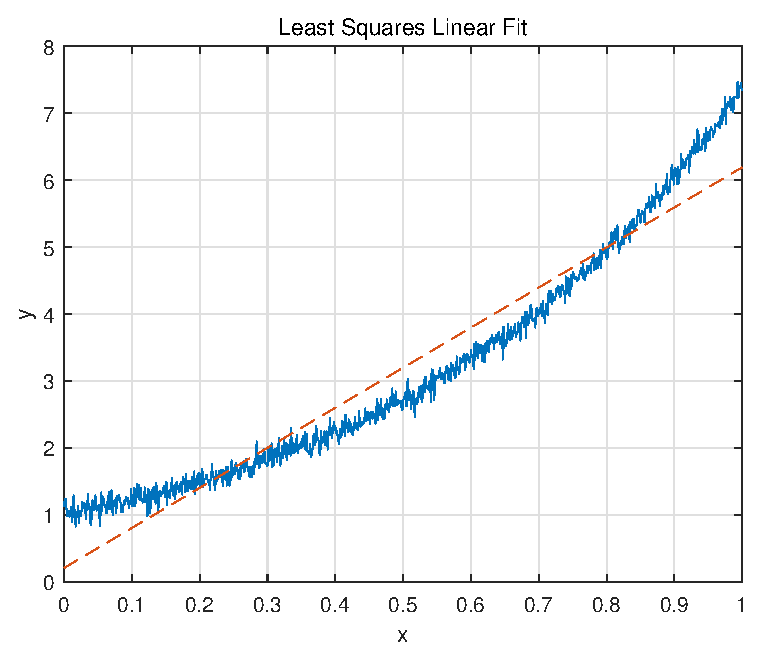
\includegraphics[scale=1]{Figure1.eps}
   \begin{center}Figure 1: plot of x(o points), x2(* points), and x4(x points)\end{center}
   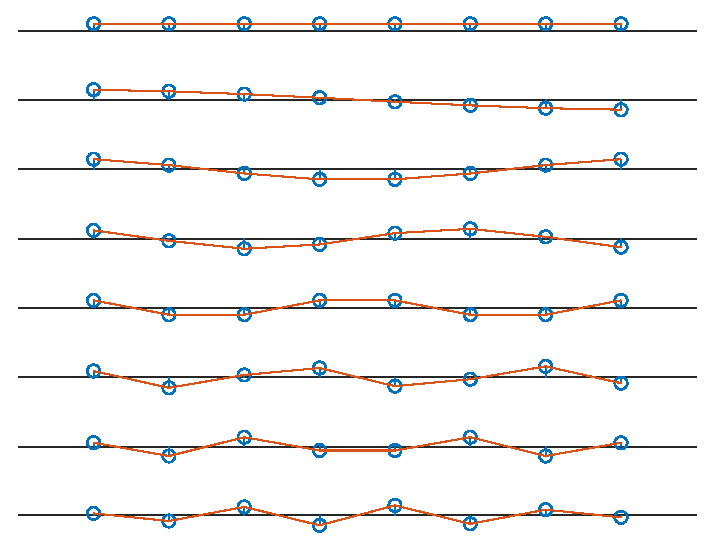
\includegraphics[scale=1]{Figure2.eps}
   \begin{center}Figure 2: 8 basis vectors of U represented by their entry values\end{center}
\end{center}
\begin{flushright}Hangshi Jin\\913142686\end{flushright}
(i)the program calculates the weights of the linear combination of the 8 basis vectors of U on x, and by using this program, we can decide which basis vectors catch the most important features of the graph of x, and then cut off the rest by setting the corresponding entries in a to 0. The decision will be made based on how much contribution each entry value does to the a in terms of its absolute value. On Figure 1, we can see how accurate the approximation has to be made in order to have a relatively similar shape to the graph of x.  Numerically, we can set a threshold based on the value of the error of each approximation to decide how accurate we want the approximation to be.
\\\\\begin{large}Problem 2\end{large}
\\\\(a)\\
\[\begin{tabular}{c|c c c c c c c c c c c}
 & D1 & D2 & D3 & D4 & D5 & D6 & D7 & D8 & D9 & D10 & D11\\
 \hline
 T1 & 0 & 1 & 0 & 0 & 1 & 1 & 0 & 0 & 0 & 0 & 0 \\\\
 T2 & 0 & 0 & 0 & 1 & 0 & 0 & 0 & 0 & 0 & 1 & 0 \\\\
 T3 & 0 & 1 & 0 & 0 & 0 & 0 & 0 & 1 & 0 & 0 & 0 \\\\
 T4 & 0 & 0 & 1 & 1 & 0 & 0 & 0 & 0 & 0 & 0 & 0 \\\\
 T5 & 0 & 0 & 0 & 1 & 0 & 0 & 0 & 0 & 0 & 1 & 0 \\\\
 T6 & 1 & 1 & 0 & 0 & 0 & 0 & 0 & 0 & 0 & 0 & 0 \\\\
 T7 & 0 & 0 & 0 & 0 & 0 & 1 & 1 & 0 & 0 & 0 & 1 \\\\
 T8 & 0 & 0 & 1 & 0 & 0 & 0 & 0 & 0 & 1 & 0 & 0 \\\\
\end{tabular}
\]
\\\\(b)
\setcounter{MaxMatrixCols}{11}
\[A=\begin{bmatrix}
0 & 1 & 0 & 0 & 1 & 1 & 0 & 0 & 0 & 0 & 0 \\
0 & 0 & 0 & 1 & 0 & 0 & 0 & 0 & 0 & 1 & 0 \\
0 & 1 & 0 & 0 & 0 & 0 & 0 & 1 & 0 & 0 & 0 \\
0 & 0 & 1 & 1 & 0 & 0 & 0 & 0 & 0 & 0 & 0 \\
0 & 0 & 0 & 1 & 0 & 0 & 0 & 0 & 0 & 1 & 0 \\
1 & 1 & 0 & 0 & 0 & 0 & 0 & 0 & 0 & 0 & 0 \\
0 & 0 & 0 & 0 & 0 & 1 & 1 & 0 & 0 & 0 & 1 \\
0 & 0 & 1 & 0 & 0 & 0 & 0 & 0 & 1 & 0 & 0
\end{bmatrix}, 
\vec{q}^{\,}=\begin{bmatrix}0\\1\\0\\1\\0\\0\\0\\0\end{bmatrix}
\]
\\\\(c)Three closest documents for q are D3,D4, and D10.
\\\\\begin{large}Problem 3\end{large}
\\\\$P_{C\rightarrow U}=$Population moved from California to elsewhere in the United States, $P_{U\rightarrow C}=$Population moved to California from another state.
\\\\\[\begin{bmatrix}
1 & -1\\
-1 & 1
\end{bmatrix}
\begin{bmatrix}
P_{C\rightarrow U}\\
P_{U\rightarrow C}
\end{bmatrix}
=\begin{bmatrix}
1 & -1\\
-1 & 1
\end{bmatrix}
\begin{bmatrix}
545921\\
458682
\end{bmatrix}
=\begin{bmatrix}
87239\\
-87239
\end{bmatrix}
\]
\begin{flushright}Hangshi Jin\\913142686\end{flushright}
\begin{large}Problem 4\end{large}
\\\\(a)
\\\\Let $v_1=x_1=\begin{bmatrix}1\\0\\1\\0\end{bmatrix}$, then\begin{equation*}v_2=x_2-proj_{w_1}x_2=\begin{bmatrix}0\\1\\0\\-1\end{bmatrix}-\frac{\begin{bmatrix}1\\0\\1\\0\end{bmatrix}\cdot\begin{bmatrix}0\\1\\0\\-1\end{bmatrix}}{\left\lVert\begin{bmatrix}1\\0\\1\\0\end{bmatrix}\right\rVert^2}\begin{bmatrix}1\\0\\1\\0\end{bmatrix}=\begin{bmatrix}0\\1\\0\\-1\end{bmatrix}\end{equation*}where $w_1$ is the space spanned by $v_1$.

\begin{equation*}v_3=x_3-proj_{w_2}x_3=\begin{bmatrix}1\\0\\0\\1\end{bmatrix}-\frac{\begin{bmatrix}1\\0\\0\\1\end{bmatrix}\cdot\begin{bmatrix}1\\0\\1\\0\end{bmatrix}}{\left\lVert\begin{bmatrix}1\\0\\1\\0\end{bmatrix}\right\rVert^2}\begin{bmatrix}1\\0\\1\\0\end{bmatrix}-\frac{\begin{bmatrix}1\\0\\0\\1\end{bmatrix}\cdot\begin{bmatrix}0\\1\\0\\-1\end{bmatrix}}{\left\lVert\begin{bmatrix}0\\1\\0\\-1\end{bmatrix}\right\rVert^2}\begin{bmatrix}0\\1\\0\\-1\end{bmatrix}=\frac{1}{2}\begin{bmatrix}1\\1\\-1\\1\end{bmatrix}\end{equation*}where $w_2$ is the space spanned by $v_1$ and $v_2$.

\begin{equation*}v_4=x_4-proj_{w_3}x_4=\begin{bmatrix}1\\1\\1\\1\end{bmatrix}-\frac{\begin{bmatrix}1\\1\\1\\1\end{bmatrix}\cdot\begin{bmatrix}1\\0\\1\\0\end{bmatrix}}{\left\lVert\begin{bmatrix}1\\0\\1\\0\end{bmatrix}\right\rVert^2}\begin{bmatrix}1\\0\\1\\0\end{bmatrix}-\frac{\begin{bmatrix}1\\1\\1\\1\end{bmatrix}\cdot\begin{bmatrix}0\\1\\0\\-1\end{bmatrix}}{\left\lVert\begin{bmatrix}0\\1\\0\\-1\end{bmatrix}\right\rVert^2}\begin{bmatrix}0\\1\\0\\-1\end{bmatrix}-\frac{1}{4}\frac{\begin{bmatrix}1\\1\\1\\1\end{bmatrix}\cdot\begin{bmatrix}1\\1\\-1\\1\end{bmatrix}}{\left\lVert\frac{1}{2}\begin{bmatrix}1\\1\\-1\\1\end{bmatrix}\right\rVert^2}\begin{bmatrix}1\\1\\-1\\1\end{bmatrix}=\frac{1}{2}\begin{bmatrix}-1\\1\\1\\1\end{bmatrix}\end{equation*}where $w_3$ is the space spanned by $v_1$, $v_2$, and $v_3$.
\\\\$\Rightarrow$The orthogonal basis is $\left\{\begin{bmatrix}1\\0\\1\\0\end{bmatrix},\begin{bmatrix}0\\1\\0\\-1\end{bmatrix},\begin{bmatrix}1\\1\\-1\\1\end{bmatrix},\begin{bmatrix}-1\\1\\1\\1\end{bmatrix}\right\}.\Rightarrow$The orthonormal basis is $\left\{\frac{\sqrt{2}}{2}\begin{bmatrix}1\\0\\1\\0\end{bmatrix},\frac{\sqrt{2}}{2}\begin{bmatrix}0\\1\\0\\-1\end{bmatrix},\frac{1}{2}\begin{bmatrix}1\\1\\-1\\1\end{bmatrix},\frac{1}{2}\begin{bmatrix}-1\\1\\1\\1\end{bmatrix}\right\}.$\\\\\\\\\\\\
\begin{flushright}Hangshi Jin\\913142686\end{flushright}
(b)
\\\\Let $u_1=y_1=\begin{bmatrix}1\\0\\1\\0\end{bmatrix}$, then \[u_2=y_2-proj_{z_1}y_2=\begin{bmatrix}4\\1\\0\\0\end{bmatrix}-\frac{\begin{bmatrix}4\\1\\0\\0\end{bmatrix}\cdot\begin{bmatrix}1\\0\\0\\1\end{bmatrix}}{\left\lVert\begin{bmatrix}1\\0\\0\\1\end{bmatrix}\right\rVert^2}\begin{bmatrix}1\\0\\0\\1\end{bmatrix}=\begin{bmatrix}2\\1\\0\\-2\end{bmatrix}\]where $z_1$ is the space spanned by $u_1$.

\begin{equation*}u_3=y_3-proj_{z_2}y_3=\begin{bmatrix}1\\0\\2\\1\end{bmatrix}-\frac{\begin{bmatrix}1\\0\\2\\1\end{bmatrix}\cdot\begin{bmatrix}1\\0\\0\\1\end{bmatrix}}{\left\lVert\begin{bmatrix}1\\0\\0\\1\end{bmatrix}\right\rVert^2}\begin{bmatrix}1\\0\\0\\1\end{bmatrix}-\frac{\begin{bmatrix}1\\0\\2\\1\end{bmatrix}\cdot\begin{bmatrix}2\\1\\0\\-2\end{bmatrix}}{\left\lVert\begin{bmatrix}2\\1\\0\\-2\end{bmatrix}\right\rVert^2}\begin{bmatrix}2\\1\\0\\-2\end{bmatrix}=\begin{bmatrix}0\\0\\2\\0\end{bmatrix}\end{equation*}where $z_2$ is the space spanned by $u_1$ and $u_2$.

\begin{equation*}u_4=y_4-proj_{z_3}y_4=\begin{bmatrix}0\\2\\0\\1\end{bmatrix}-\frac{\begin{bmatrix}0\\2\\0\\1\end{bmatrix}\cdot\begin{bmatrix}1\\0\\0\\1\end{bmatrix}}{\left\lVert\begin{bmatrix}1\\0\\0\\1\end{bmatrix}\right\rVert^2}\begin{bmatrix}1\\0\\0\\1\end{bmatrix}-\frac{\begin{bmatrix}0\\2\\0\\1\end{bmatrix}\cdot\begin{bmatrix}2\\1\\0\\-2\end{bmatrix}}{\left\lVert\begin{bmatrix}2\\1\\0\\-2\end{bmatrix}\right\rVert^2}\begin{bmatrix}2\\1\\0\\-2\end{bmatrix}-\frac{\begin{bmatrix}0\\2\\0\\1\end{bmatrix}\cdot\begin{bmatrix}0\\0\\2\\0\end{bmatrix}}{\left\lVert\frac{1}{2}\begin{bmatrix}0\\0\\2\\0\end{bmatrix}\right\rVert^2}\begin{bmatrix}0\\0\\2\\0\end{bmatrix}=\frac{1}{2}\begin{bmatrix}-1\\4\\0\\1\end{bmatrix}\end{equation*}where $z_3$ is the space spanned by $u_1$, $u_2$, and $u_3$.
\\\\$\Rightarrow$The orthogonal basis is $\left\{\begin{bmatrix}1\\0\\0\\1\end{bmatrix},\begin{bmatrix}2\\1\\0\\-2\end{bmatrix},\begin{bmatrix}0\\0\\2\\0\end{bmatrix},\begin{bmatrix}-1\\4\\0\\1\end{bmatrix}\right\}$.$\Rightarrow$The orthonormal basis is $\left\{\frac{\sqrt{2}}{2}\begin{bmatrix}1\\0\\0\\1\end{bmatrix},\frac{1}{3}\begin{bmatrix}2\\1\\0\\-2\end{bmatrix},\begin{bmatrix}0\\0\\1\\0\end{bmatrix},\frac{\sqrt{2}}{6}\begin{bmatrix}-1\\4\\0\\1\end{bmatrix}\right\}$.\\\\\\\\\\\\\\\\
\begin{flushright}Hangshi Jin\\913142686\end{flushright}
\begin{large}Problem 5\end{large}
\\\\(a)Domain of T is $R^4$, and codomain of T is $R^7$.
\\\\(b)\[C(A)=span\left\{\begin{bmatrix}1\\0\\0\\0\\0\\0\\0\end{bmatrix},\begin{bmatrix}2\\1\\0\\0\\0\\0\\0\end{bmatrix},\begin{bmatrix}3\\5\\1\\0\\0\\0\\0\end{bmatrix},\begin{bmatrix}4\\7\\6\\1\\0\\0\\0\end{bmatrix}\right\}\]
\\\\(c)\[A=\begin{bmatrix}
1 & 2 & 3 & 4\\
0 & 1 & 5 & 7\\
0 & 0 & 1 & 6\\
0 & 0 & 0 & 1\\
0 & 0 & 0 & 0\\
0 & 0 & 0 & 0\\
0 & 0 & 0 & 0
\end{bmatrix}\xrightarrow{\begin{matrix}r_1-2r_2\end{matrix}}
\begin{bmatrix}
1 & 0 & -7 & -10\\
0 & 1 & 5 & 7\\
0 & 0 & 1 & 6\\
0 & 0 & 0 & 1\\
0 & 0 & 0 & 0\\
0 & 0 & 0 & 0\\
0 & 0 & 0 & 0
\end{bmatrix}\xrightarrow{\begin{matrix}r_1+7r_3\\r_2-5r_3\end{matrix}}
\begin{bmatrix}
1 & 0 & 0 & 32\\
0 & 1 & 0 & -23\\
0 & 0 & 1 & 6\\
0 & 0 & 0 & 1\\
0 & 0 & 0 & 0\\
0 & 0 & 0 & 0\\
0 & 0 & 0 & 0
\end{bmatrix}\xrightarrow{\begin{matrix}r_1-32r_4\\r_2+23r_4\\r_3-6r_4\end{matrix}}
\begin{bmatrix}
1 & 0 & 0 & 0\\
0 & 1 & 0 & 0\\
0 & 0 & 1 & 0\\
0 & 0 & 0 & 1\\
0 & 0 & 0 & 0\\
0 & 0 & 0 & 0\\
0 & 0 & 0 & 0
\end{bmatrix}=rref(A)
\] 
\[\Rightarrow B_{C(A)}=\left\{\begin{bmatrix}1\\0\\0\\0\\0\\0\\0\end{bmatrix},\begin{bmatrix}2\\1\\0\\0\\0\\0\\0\end{bmatrix},\begin{bmatrix}3\\5\\1\\0\\0\\0\\0\end{bmatrix},\begin{bmatrix}4\\7\\6\\1\\0\\0\\0\end{bmatrix}\right\}
\]
\\\\(d)	\[N(A)=span\begin{bmatrix}0\\0\\0\\0\end{bmatrix}=\vec{0}^{\,}\]
\\\\(e)\[B_{N(A)}=\left\{\vec{0}^{\,}\right\}\]
\\\\(f)\[row(A)=span\left\{\begin{bmatrix}1&2&3&4\end{bmatrix},\begin{bmatrix}0&1&5&7\end{bmatrix},\begin{bmatrix}0&0&1&6\end{bmatrix},\begin{bmatrix}0&0&0&1\end{bmatrix}\right\}\]\\\\\\
\begin{flushright}Hangshi Jin\\913142686\end{flushright}
(g)\[A^T=\begin{bmatrix}
1&0&0&0&0&0&0\\
2&1&0&0&0&0&0\\
3&5&1&0&0&0&0\\
4&7&6&1&0&0&0	
\end{bmatrix}\Rightarrow N(A^T)=\left\{\begin{bmatrix}0\\0\\0\\0\\1\\0\\0\end{bmatrix},\begin{bmatrix}0\\0\\0\\0\\0\\1\\0\end{bmatrix},\begin{bmatrix}0\\0\\0\\0\\0\\0\\1\end{bmatrix}\right\}\]
\\\\(h)\[rank(A)=4\]
\\\\\begin{large}Problem 5\end{large}
\\\\(a)(i)$11111 = (1 \cdot 2^4) + (1 \cdot 2^3) + (1 \cdot 2^2) + (1 \cdot 2^1) + (1 \cdot 2^0) = 31$
\\\\(ii)$1000000 = (1 \cdot 2^6) + (0 \cdot 2^5) + (0 \cdot 2^4) + (0 \cdot 2^3) + (0 \cdot 2^2) + (0 \cdot 2^1) + (0 \cdot 2^0) = 64$
\\\\(iii)$1001101101 = (1 \cdot 2^9) + (0 \cdot 2^8) + (0 \cdot 2^7) + (1 \cdot 2^6) + (1 \cdot 2^5) + (0 \cdot 2^4) + (1 \cdot 2^3) + (1 \cdot 2^2) + (0 \cdot 2^1) + (1 \cdot 2^0) = 621$
\\\\(iv)$10101010 = (1 \cdot 2^7) + (0 \cdot 2^6) + (1 \cdot 2^5) + (0 \cdot 2^4) + (1 \cdot 2^3) + (0 \cdot 2^2) + (1 \cdot 2^1) + (0 \cdot 2^0) = 170$
\\\\(v)$000011110000 = (0 \cdot 2^{11}) + (0 \cdot 2^{10}) + (0 \cdot 2^9) + (0 \cdot 2^8) + (1 \cdot 2^7) + (1 \cdot 2^6) + (1 \cdot 2^5) \\\\+ (1 \cdot 2^4) + (0 \cdot 2^3) + (0 \cdot 2^2) + (0 \cdot 2^1) + (0 \cdot 2^0) = 240$
\\\\(b)(i)\[\begin{tabular}{|c|c|c|c|}
\hline
\text{Division by 2}&\text{Quotient}&\text{Remainder}&\text{Bit Number}\\
\hline
$73/2$&36&1&0\\
\hline
$36/2$&18&0&1\\
\hline
$18/2$&9&0&2\\
\hline
$9/2$&4&1&3\\
\hline
$4/2$&2&0&4\\
\hline
$2/2$&1&0&5\\
\hline
$1/2$&0&1&6\\
\hline
\end{tabular}\]
$\Rightarrow$1001001
\\\\(b)(ii)\[\begin{tabular}{|c|c|c|c|}
\hline
\text{Division by 2}&\text{Quotient}&\text{Remainder}&\text{Bit Number}\\
\hline
$127/2$&63&1&0\\
\hline
$63/2$&31&1&1\\
\hline
$31/2$&15&1&2\\
\hline
$15/2$&7&1&3\\
\hline
$7/2$&3&1&4\\
\hline
$3/2$&1&1&5\\
\hline
$1/2$&0&1&6\\
\hline
\end{tabular}\]
$\Rightarrow$1111111\\\\
\begin{flushright}Hangshi Jin\\913142686\end{flushright}
(b)(iii)\[\begin{tabular}{|c|c|c|c|}
\hline
\text{Division by 2}&\text{Quotient}&\text{Remainder}&\text{Bit Number}\\
\hline
$402/2$&201&0&0\\
\hline
$201/2$&100&1&1\\
\hline
$100/2$&50&0&2\\
\hline
$50/2$&25&0&3\\
\hline
$25/2$&12&1&4\\
\hline
$12/2$&6&0&5\\
\hline
$6/2$&3&0&6\\
\hline
$3/2$&1&1&6\\
\hline
$1/2$&0&1&6\\
\hline
\end{tabular}\]
$\Rightarrow$110010010
\\\\(b)(iv)\[\begin{tabular}{|c|c|c|c|}
\hline
\text{Division by 2}&\text{Quotient}&\text{Remainder}&\text{Bit Number}\\
\hline
$512/2$&256&0&0\\
\hline
$256/2$&128&0&1\\
\hline
$128/2$&64&0&2\\
\hline
$64/2$&32&0&3\\
\hline
$32/2$&16&0&4\\
\hline
$16/2$&8&0&5\\
\hline
$8/2$&4&0&6\\
\hline
$4/2$&2&0&6\\
\hline
$2/2$&1&0&6\\
\hline
\end{tabular}\]
$\Rightarrow$1000000000
\\\\(b)(v)\[\begin{tabular}{|c|c|c|c|}
\hline
\text{Division by 2}&\text{Quotient}&\text{Remainder}&\text{Bit Number}\\
\hline
$1000/2$&500&0&0\\
\hline
$500/2$&250&0&1\\
\hline
$250/2$&125&0&2\\
\hline
$125/2$&62&1&3\\
\hline
$62/2$&31&0&4\\
\hline
$31/2$&15&1&5\\
\hline
$15/2$&7&1&6\\
\hline
$7/2$&3&1&6\\
\hline
$3/2$&1&1&6\\
\hline
$1/2$&0&1&7\\
\hline
\end{tabular}\]
$\Rightarrow$1111101000
\\\\\\\\\\\\\\\\\\\\\begin{flushright}Hangshi Jin\\913142686\end{flushright}(b)(vi)\[\begin{tabular}{|c|c|c|c|}
\hline
\text{Division by 2}&\text{Quotient}&\text{Remainder}&\text{Bit Number}\\
\hline
$32767/2$&16383&1&0\\
\hline
$16383/2$&8191&1&1\\
\hline
$8191/2$&4095&1&2\\
\hline
$4095/2$&2047&1&3\\
\hline
$2047/2$&1023&1&4\\
\hline
$1023/2$&511&1&5\\
\hline
$511/2$&255&1&6\\
\hline
$255/2$&127&1&6\\
\hline
$127/2$&63&1&6\\
\hline
$63/2$&31&1&6\\
\hline
$31/2$&15&1&6\\
\hline
$15/2$&7&1&6\\
\hline
$7/2$&3&1&6\\
\hline
$3/2$&1&1&6\\
\hline
$1/2$&0&1&6\\
\hline
\end{tabular}\]
$\Rightarrow$111111111111111
\end{document}